\chapter{Ausgangssituation und Zielsetzung}

\section{Ausgangssituation}
Die HTBLA-Leonding ist eine BHS im Raum Oberösterreich, welche für ihre gute Ausbildung und interessanten Projekte im Bereich der Informationstechnologie bekannt ist.

\section{Beschreibung des Problembereichs}
In den Klassenräumen fehlt es oft an Sauerstoff, manchmal ist auch die Temperatur nicht adäquat. Dieseh kann eine Reihe von unerwünschten Symptomen hervorrufen, wie zum Beispiel: 

\begin{itemize}
    \item Kopfschmerzen
    \item Ermüdung
    \item Schwindel
    \item Übelkeit
    \item mehr Probleme mit Asthma und Allergien
\end{itemize}

Die oben gennannten Symptome sind in einer Umgebung wie der Schule unbedingt zu vermeiden, da es ansonsten zu einem Konzentrationsverlust der Schüler führt.

Um zusätzlich eine Regelung der Heizung vornehmen zu können sind weitere Informationen der einzelnen Klassenräume, wie die Temperatur, notwendig. Weiters wird es rund um die Uhr ermöglicht,  geöffnete Fenster zu lokalisieren und mit dieser Information Schäden an der Schule zu verhindern.

\section{Aufgabenstellung}
Um Sensoren in der Schule platzieren zu können, ist es erforderlich, zuerst eine Mesh-Infrastruktur für die Auswertung der Sensoren zu gestalten.

Eine Einbindung eines MQTT-Netzwerkes, welches direkt auf dem Mesh-Netzwerk aufsitzt ist ebenso notwendig. Dieses Mesh-Netzwerk ermöglicht den verschiedenen Knoten, welche mit den Sensoren und Aktoren verbunden sind, untereinander zu komunizieren und Informationen auszutauschen.

Um den Überblick über solch ein Netzwerk nicht zu verlieren, ist es ebenso wünschenswert eine Visualisierungs-Komponente zu gestallten, welche es ermöglicht den aktuellen Zustandes des Mesh-Netzwerkes zu inspizieren und den Benutzer nachvollziehen lässt wann Nachrichten versendet werden.

Zusätzlich dazu soll ein System entwickelt werden, welches es ESPs ermöglicht OTA Updates durchzuführen.

\begin{figure}[H]
    \centering
    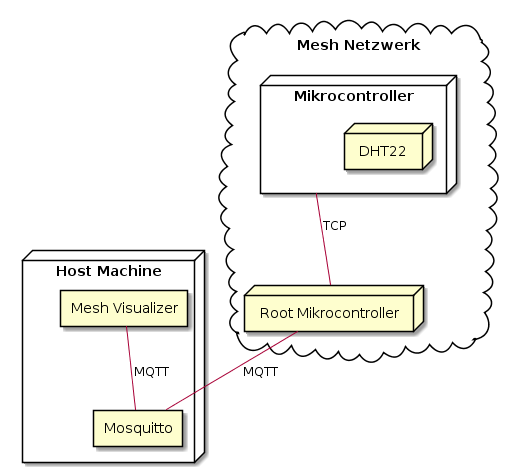
\includegraphics[scale=0.7]{diagrams/deployment.png}
    \caption{Systemarchitektur (Quelle: Eigene Darstellung)}
    \label{abb:deployment}
\end{figure}

\section{Zielbestimmung}
Das Ziel dieses System ist es die, den Schülern eine stress- und sorgenfreie Lernumgebung zu ermöglichen.